\chapter{Objet}

Ce document a pour but de présenter l'architecture technique de ce projet. Le but de ce projet est de développer un outil de protection et de gestion des licences.

\chapter{Documents de référence}

Documents de spécification :

\begin{itemize}
    \item Spécification Technique des Besoins
    \item Fiches techniques :
	\begin{itemize}
	    \item Injection de code dans un PE
	    \item Génération de licence
	    \item Signature
	    \item Obfuscation de code
	    \item Sécurisation des bases de données
	\end{itemize}
\end{itemize}

\chapter{Terminologie}

\chapter{Configuration requise}

Les éléments matériels nécessaire au développement de cet outil sont :

\begin{itemize}
    \item Un serveur
\end{itemize}

\chapter{Architecture statique}
Afin de réaliser ce projet nous avons choisit de mettre en place l'infrastructure suivante:
\begin{itemize}
	\item Un serveur web qui permettra
	\begin{itemize}
		\item a un client de se créer un compte, demander et télécharger l'outil de generation
					de licence.
		\item a un administrateur d'accorder et de gérer les licences. 
	\end{itemize}
	\item Un logiciel d'activation qui sera executé sur la machine de l'utilisateur
				afin de lui permettre de générer une licence. Pour cela il échangera avec
				le serveur des informations sur le matériel physique de la machine, ce 
				qui permettra à ce dernier de générer le fichier de licence.
	\item Un outil permettant de vérifier la validité d'une licence, cette outil
				pourra prendre les formes suivantes: 
	\begin{itemize}
	\item Une bibilothèque de fonction qui permettra à un developpeur d'inclure
				dans son code les fonctions de vérification de licence. 
	\item Un programme permettant de greffer directement les fonctions de vérification
				sur un exécutable. 
	\end{itemize}
\end{itemize}
L'architecture générale de ce projet peut être représenter via le schéma n°\ref{fig:fig1}\newline
\begin{figure}[h!]
	\centering
	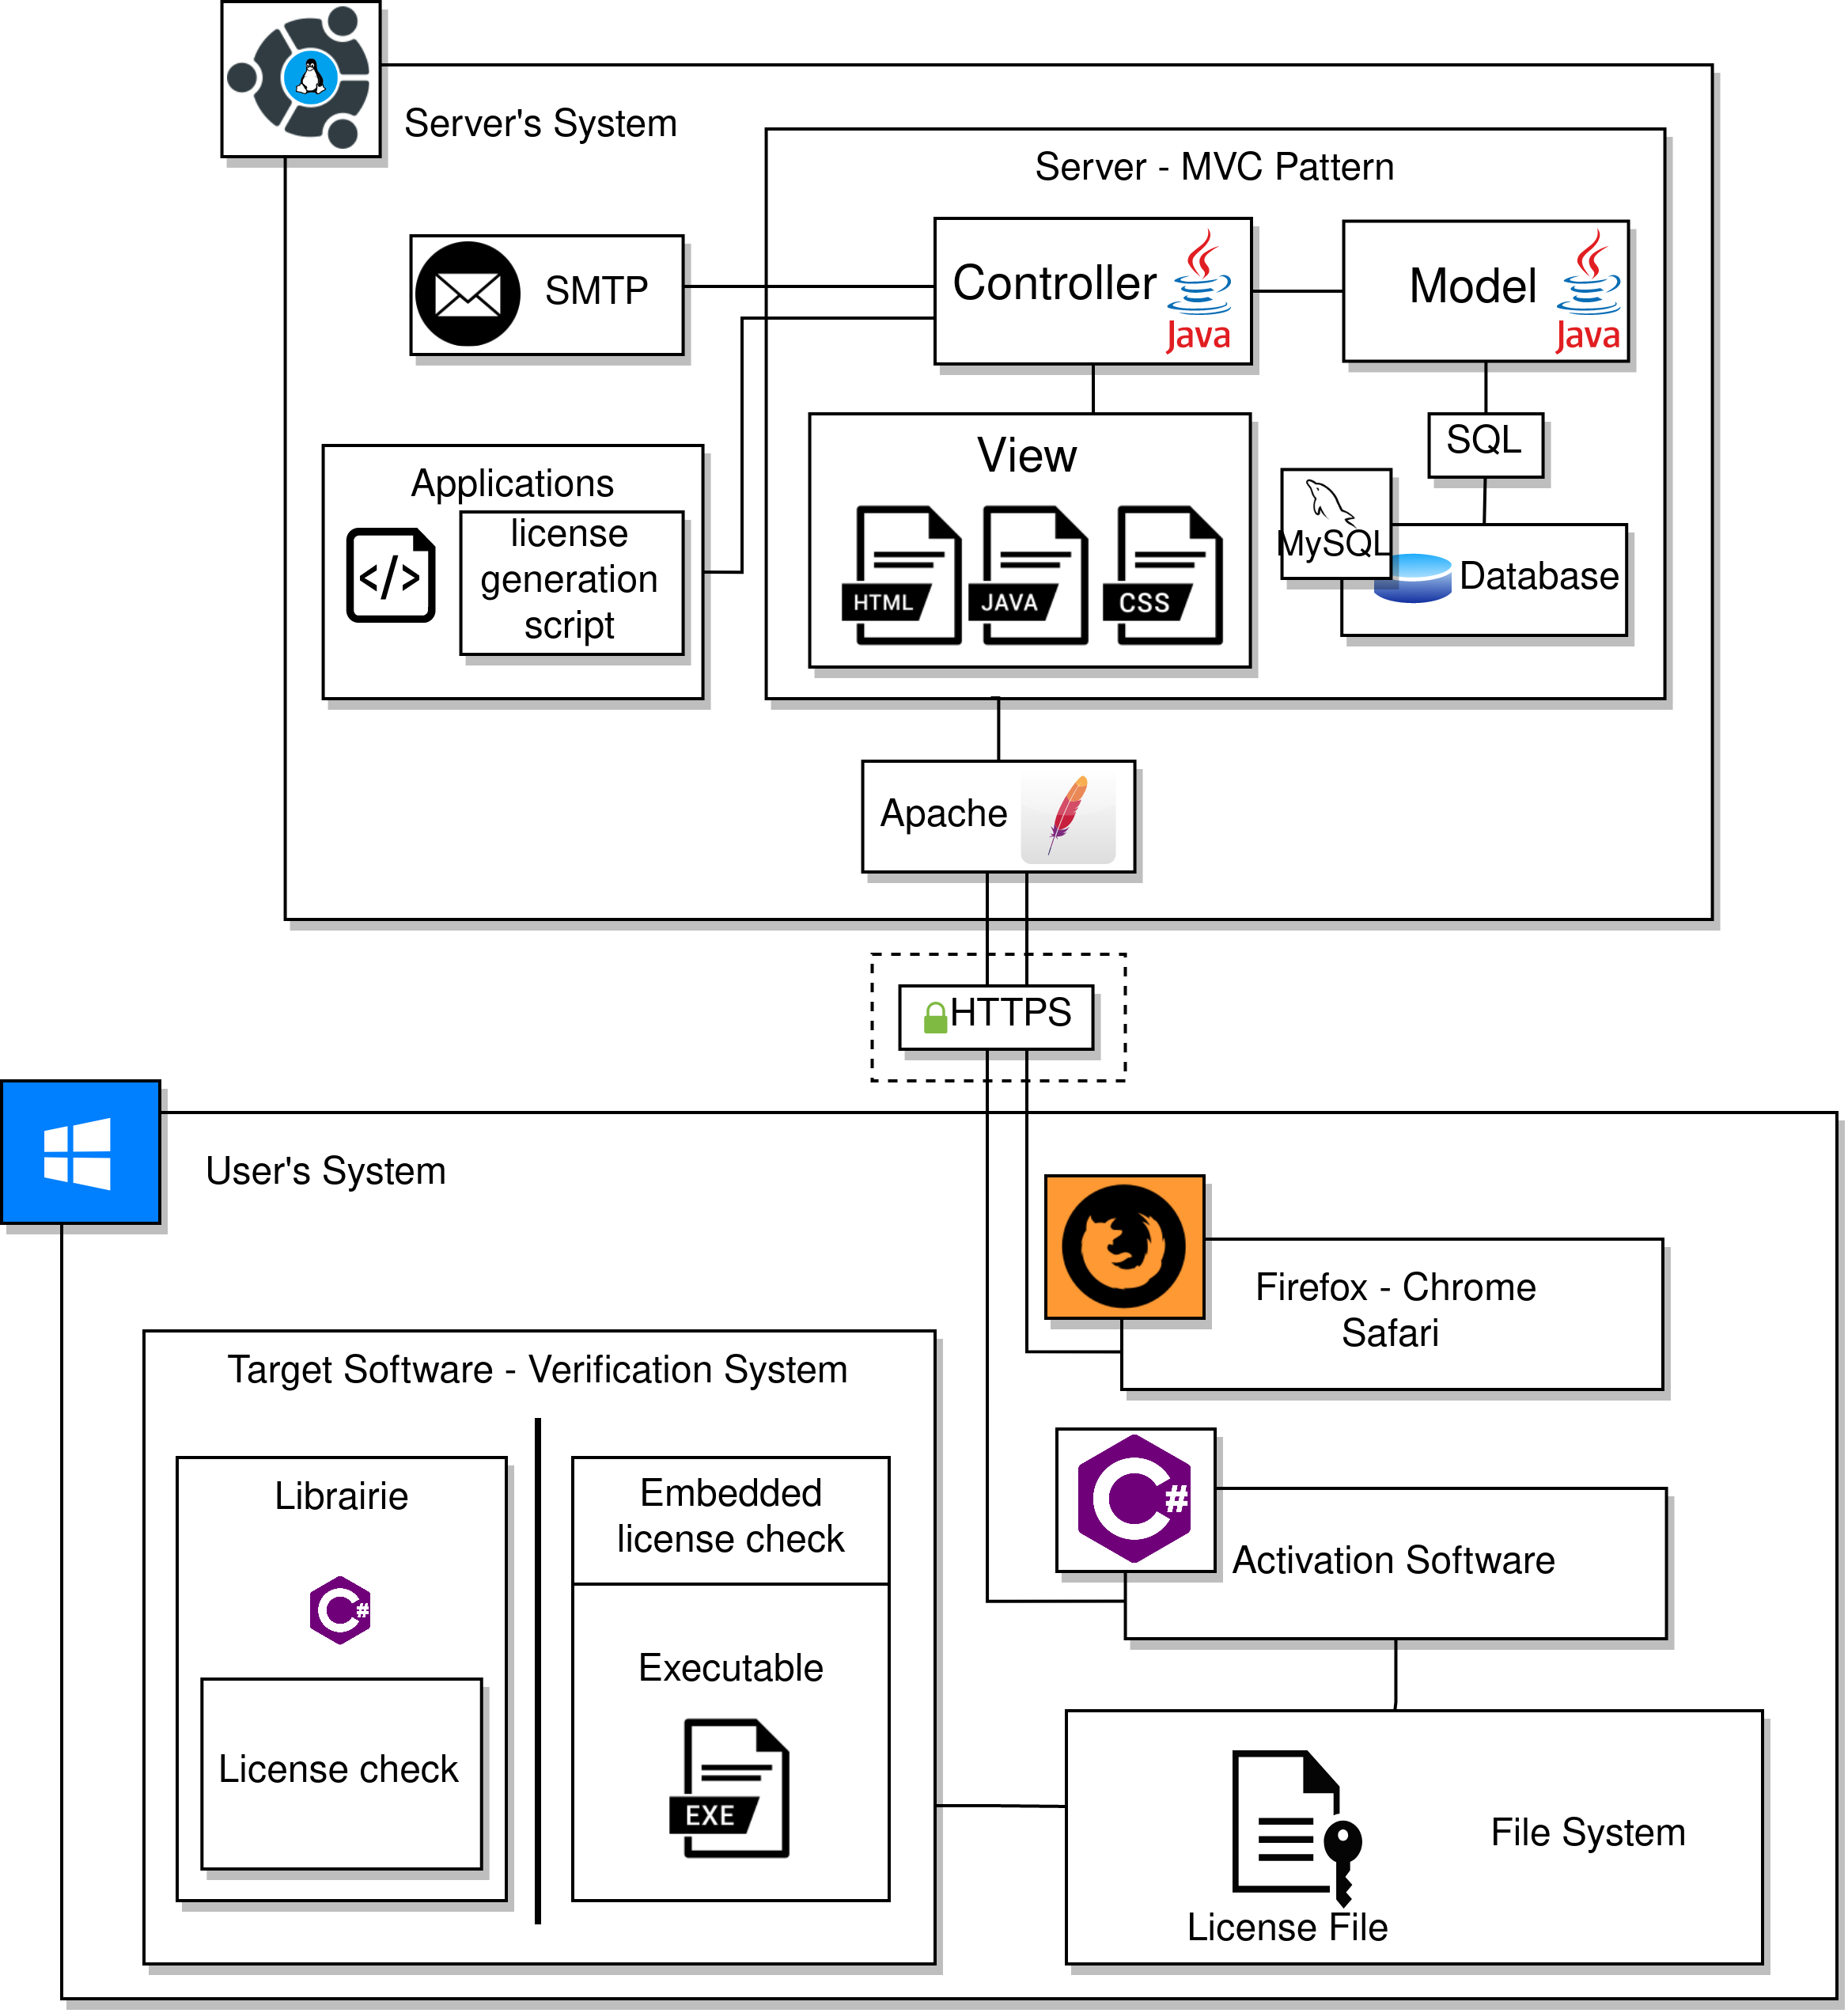
\includegraphics{../png/DAT_general.png}
	\caption{Schéma d'architecture générale}
	\label{fig:fig1}
\end{figure}
\newpage

\section{Constituant 'Serveur'}
\subsection{Description}
\begin{itemize}
	\item Le but du serveur est de fournir l'interface principale, programmé 
				en HTML, CSS et JS aux utilisateurs, de stocker dans sa base de donnée
				les informations nécessaires à la génération de licence et enfin de générer 
				les licences.
	\item Propriétés et attributs de caractérisation
	\item Services offerts (interfaces)
	\item Dépendances avec d’autres constituants (services utilisés, composants 'étagère' utilisés)
	\item HTML, CSS, JS, PHP, SQL, Bash 
	\item Architecture MVC (Model Vue Controler)
	\item Taille importante et complexité élévé.
\end{itemize}
\subsection{Justifications techniques.}

\section{Constituant 'Logiciel d'Activation'}
\subsection{Description}
\begin{itemize}
	\item Récuperer les informations matériels sur la machine d'un utilisateur, puis 
				se connecter au serveur afin de générer le fichier de licence.
	\item Propriétés et attributs de caractérisation
	\item Services offerts (interfaces)
	\item Dépendances avec d’autres constituants (services utilisés, composants 'étagère' utilisés)
	\item C\# ?
	\item Procédé de développement (techniques, méthodes et/ou outils )
	\item Taille et complexité.
\end{itemize}
\subsection{Justifications techniques.}

\section{Constituant 'Système de véfication - Librairie'}
\subsection{Description}
\begin{itemize}
	\item Fournir une API pour des programmes en C\# afin de 
				permettre à un developpeur de vérifier une licence dans son code.
	\item Propriétés et attributs de caractérisation
	\item Listes des fonctions de l'API (a faire)
	\item Dépendances avec d’autres constituants (services utilisés, composants 'étagère' utilisés)
	\item C, C++, C\#
	\item Procédé de développement (techniques, méthodes et/ou outils )
	\item Taille et complexité.
\end{itemize}
\subsection{Justifications techniques.}

\section{Constituant 'Système de véfication - Greffe'}
\subsection{Description}
\begin{itemize}
	\item Outil permettant d'ajouter les fonctions de vérification directement à un
				executable, afin de décharger le developpeur de la necessité de vérifier 
				la licence dans son code.
	\item Propriétés et attributs de caractérisation
	\item Services offerts (interfaces)
	\item Dépendances avec d’autres constituants (services utilisés, composants 'étagère' utilisés)
	\item C, C\#, Python, Bash 
	\item Procédé de développement (techniques, méthodes et/ou outils )
	\item Taille et complexité.
\end{itemize}
\subsection{Justifications techniques.}

